\chapter{Конструкторский раздел}

В конструкторской части были разработаны реляционная схема базы данных и ролевая модель, рассмотрены ограничения целостности и разработана процедура


\section{Схема базы данных}
В аналитической части была выбрана реляционная модель данных, поэтому данные организованы в виде связных таблиц. На рисунке~\ref{img:scheme} представлена реляционная схема базы данных, основанная на диаграмме сущность-связь~\ref{img:er}, отражающей структуру базы данных и связи между сущностями.

\begin{figure}[H]
    \centering
    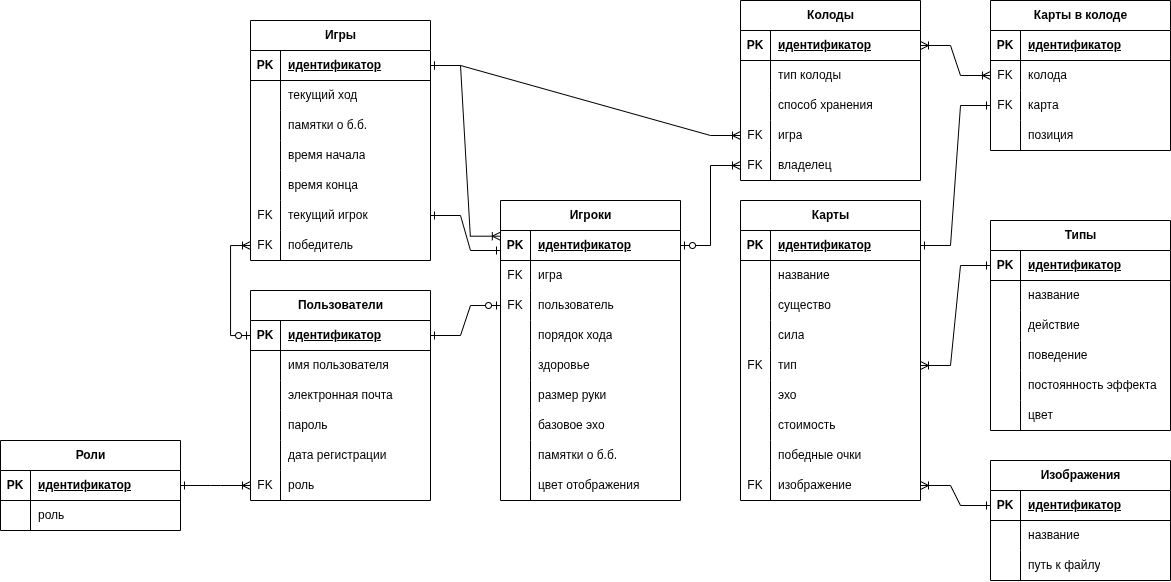
\includegraphics[width=1\linewidth]{../img/relational-db-scheme}
    \caption{Реляционная схема базы данных}
    \label{img:scheme}
\end{figure}


\section{Ограничения целостности}
Введены следующие ограничения на данные для соблюдения целостности данных:

\begin{itemize}

    \item победитель партии может быть указан только для завершённой партии;
    
    \item в рамках одной партии у одного игрока не должно быть более одной колоды каждого личного типа: колоды добора, руки, стола и сброса;

    \item в рамках одной партии не должно быть более одной открытой колоды рынка, одной закрытой колоды рынка и одной колоды игрового сброса;

    \item купить можно только карту, находящуюся в открытом рынке текущей партии;

  	\item покупка карты возможна только при наличии у игрока достаточного количества эхо;
    
    \item после покупки карта должна быть удалена из открытого рынка и добавлена в сброс игрока;
    
   	\item игрок может разыгрывать только карты, находящиеся в его руке, и только в свой ход;
   
   	\item после розыгрыша карта удаляется из руки игрока и помещается на стол;
   
   	\item при завершении хода игрока все карты из руки и со стола перемещаются в сброс игрока, после чего формируется новая рука из колоды добора.

	\item если количество оставшихся памяток о бренности бытия становится равным нулю, партия должна перейти в завершённое состояние.

\end{itemize}


\section{Нормальная форма}
База данных должна удовлетворять 3НФ.

Первая нормальная форма соблюдается, так как все атрибуты отношений являются атомарными. Например, список карт, находящихся в колоде, не хранится в одном поле внутри $decks$, а вынесен в отдельное отношение $deck\_cards$. Каждая строка $deck\_cards$ описывает одно вхождение карты в одну колоду.

Вторая нормальная форма требует, чтобы отношение находилось в первой нормальной форме, а каждый неключевой атрибут полностью зависел от всего первичного ключа, а не от его части. В разработанной схеме базы данных составные первичные ключи не используются, каждое отношение имеет простой первичный ключ $id$. Все отношения схемы, находящиеся в первой нормальной форме, удовлетворяют требованиям второй нормальной формы.

Третья нормальная форма требует, чтобы отношение находилось во второй нормальной форме и не содержало транзитивных зависимостей неключевых атрибутов от ключа через другие неключевые атрибуты. Для выполнения этого требования справочные и повторяющиеся данные были вынесены в отдельные отношения~\cite{date}.


\section{Проектирование хранимой процедуры покупки карты}

Для выполнения операции покупки карты с открытого рынка в базе реализована хранимая процедура $buy\_card\_from\_market$. Она используется для того, чтобы все проверки и все изменения происходили вместе. 

Атомарность операции покупки карты обеспечивается механизмом транзакций СУБД. Все изменения данных выполняются в рамках одной транзакции. В случае возникновения ошибки на любом этапе выполнения процедуры формируется исключение, что приводит к откату транзакции. Таким образом, либо все изменения (списание эхо, удаление карты из рынка и добавление карты в сброс) выполняются полностью, либо не выполняется ни одно из них.

Транзакционность операции обеспечивается тем, что выполнение хранимой процедуры происходит в рамках одной транзакции СУБД. Все проверки и изменения состояния выполняются последовательно и фиксируются только при успешном завершении процедуры. В случае возникновения ошибки транзакция откатывается.

Схема хранимой процедуры представлена на рисунке~\ref{img:buy_market_card}.

\begin{figure}[H]
    \centering
    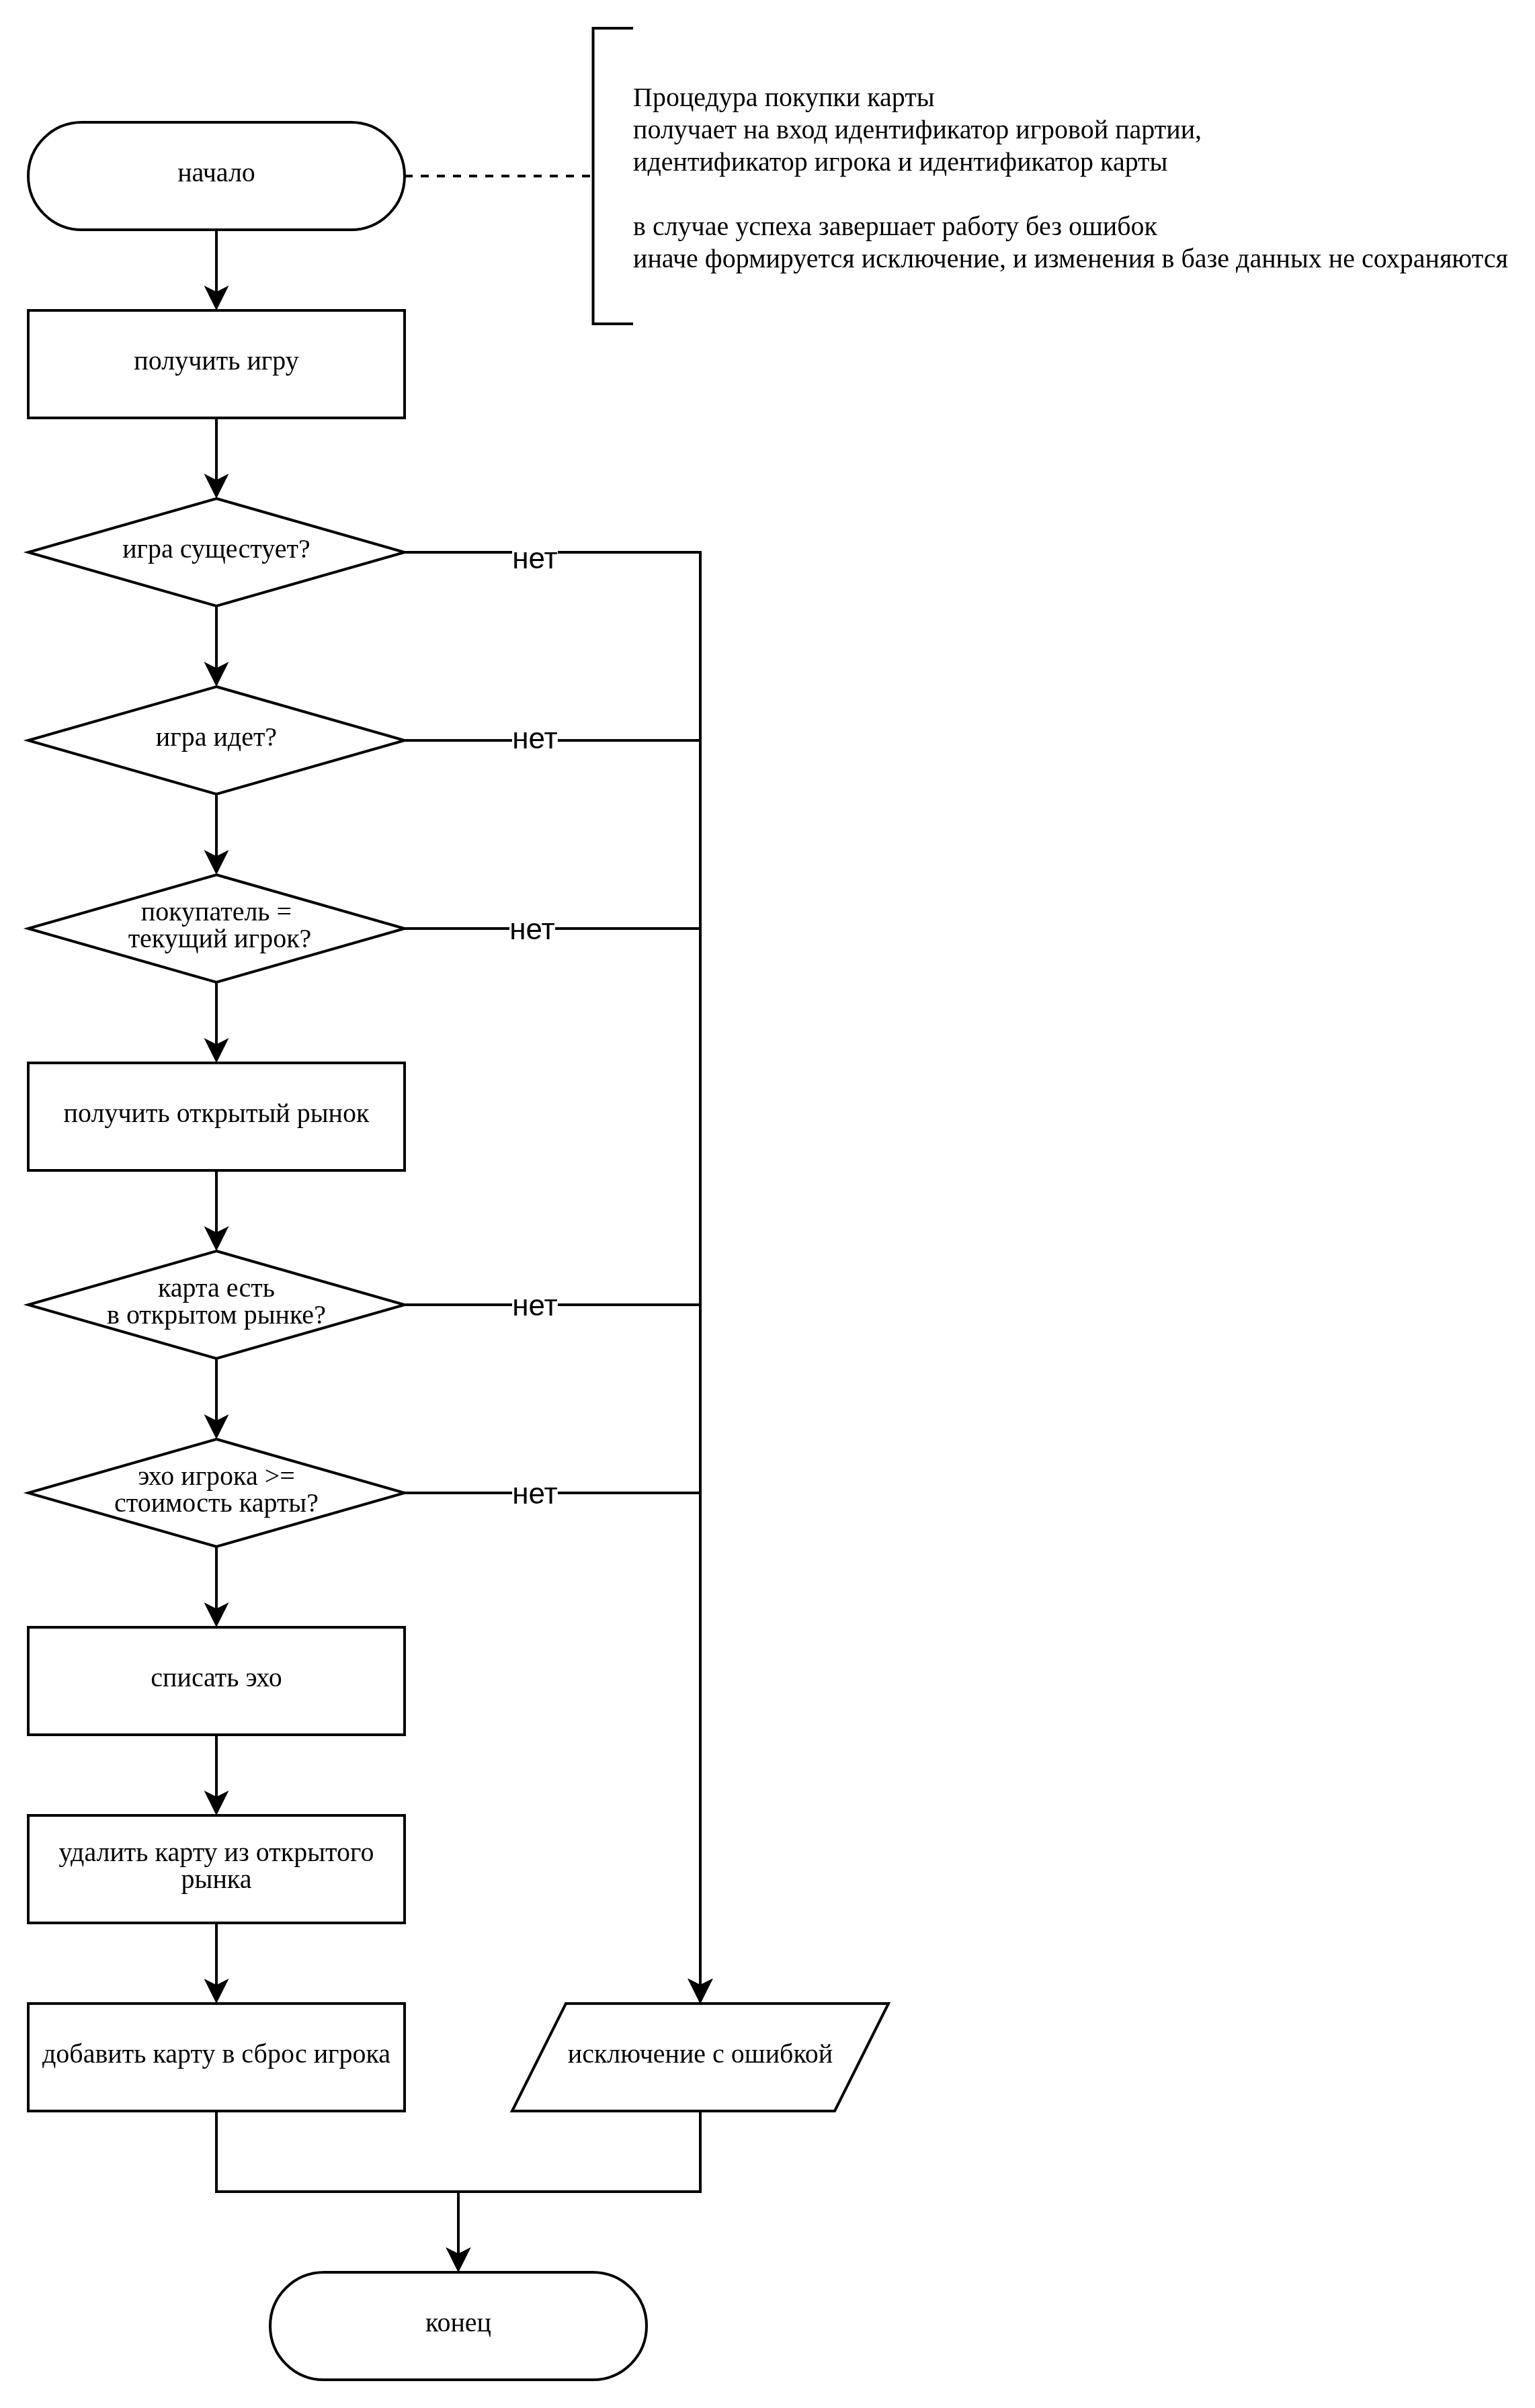
\includegraphics[width=0.9\linewidth]{../img/card_buy_procedure}
    \caption{Схема хранимой процедуры покупки карты из открытого рынка}
    \label{img:buy_market_card}
\end{figure}


\section{Проектирование триггера}

Для поддержания целостности данных необходимо, чтобы тип колоды соответствовал её владельцу. Личные колоды игрока, такие как колода добора, рука, стол и сброс, должны принадлежать конкретному игроку. Общие колоды партии, такие как открытый рынок, закрытый рынок и общий игровой сброс, не должны иметь владельца --- они принадлежат игре напрямую.

Для проверки этого ограничения используется триггер, который срабатывает перед добавлением или изменением записи в таблице \texttt{decks}. Триггер проверяет тип колоды, наличие владельца и соответствие партии колоды партии игрока.

Схема работы такого триггера представлена на рисунке~\ref{img:trigger}.

\begin{figure}[H]
    \centering
    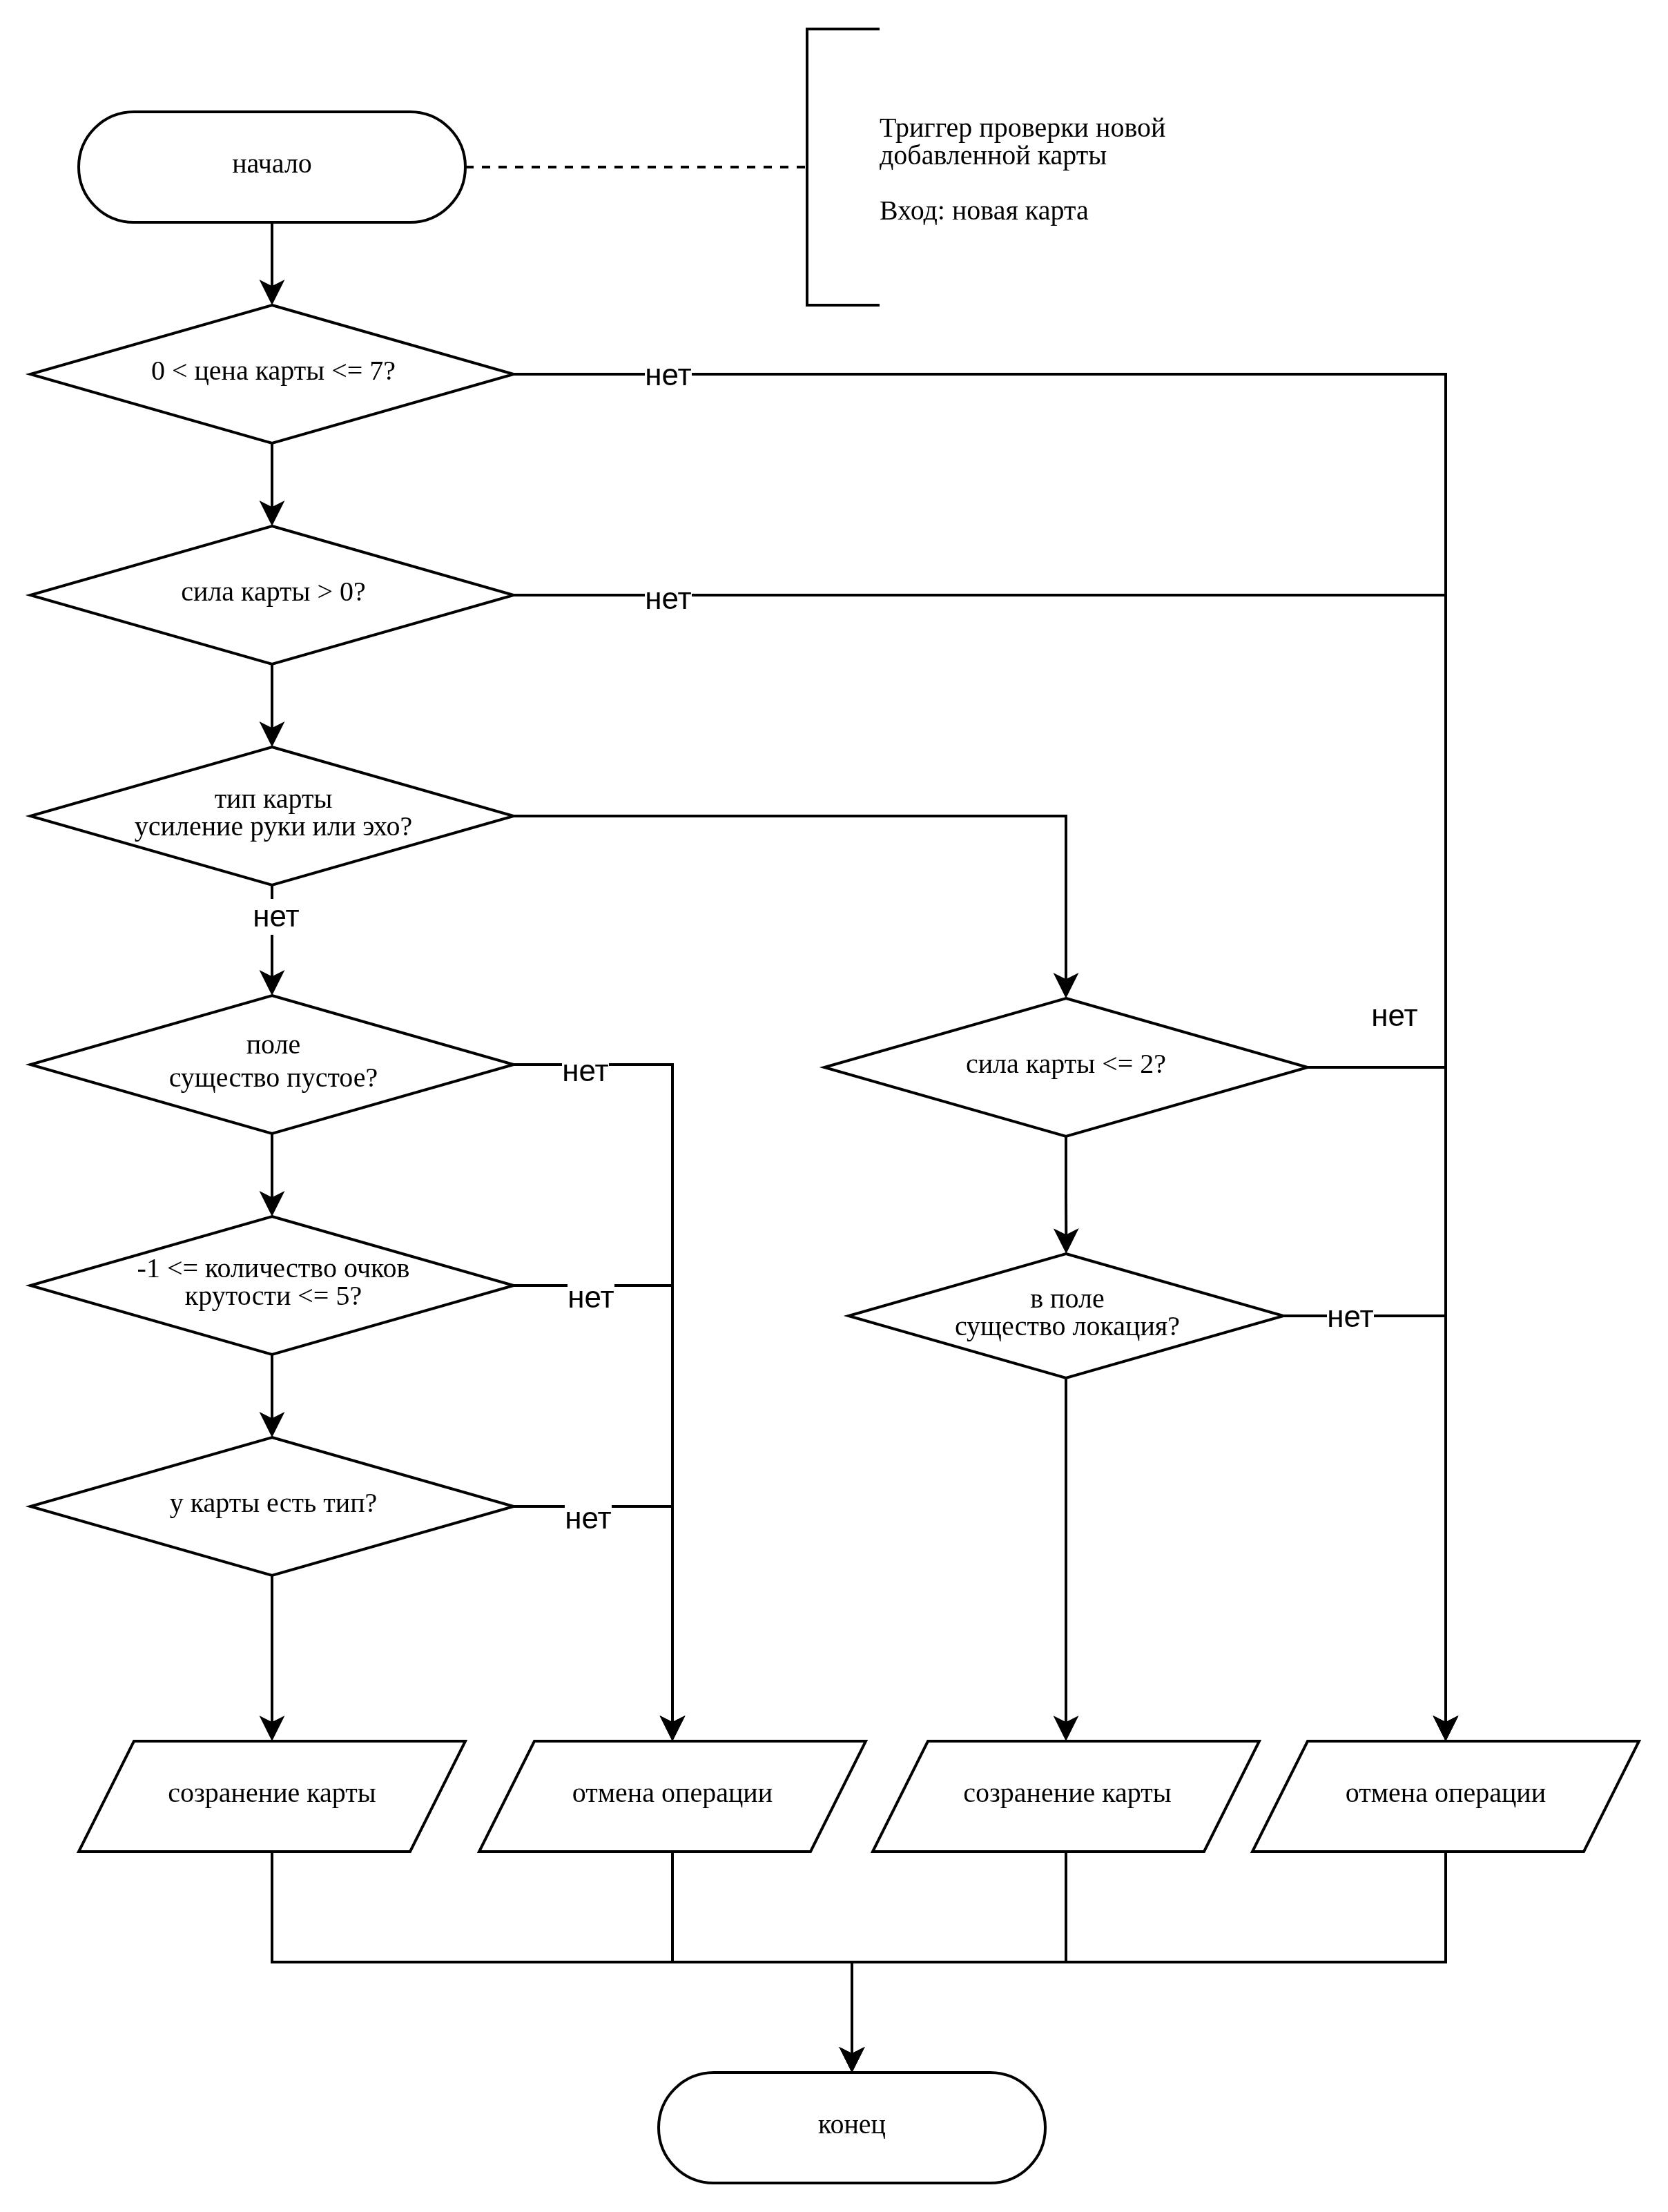
\includegraphics[width=0.7\linewidth]{../img/card_check_trigger}
    \caption{Схема триггера проверки владельца колоды}
    \label{img:trigger}
\end{figure}


\section{Ролевая модель}

На основе пользователей приложения, описанных в аналитической части, были сформированы следующие роли и права доступа к базе данных:
\begin{itemize}
    \item пользователь (гость) --- имеет доступ к каталогу игровых карт и правилам;
    \item авторизованный пользователь --- так же может просматривать и создавать записи в таблице игровых партий;
    \item игрок --- имеет доступ к просмотру, изменению записей таблиц игровых колод и просмотру таблицы игроков в игре;
    \item модератор --- обладает всеми правами авторизованного пользователя и может изменять и удалять записи в таблицах пользователей и игровых партий;
    \item мастер --- всё то же, что и модератор, а также изменение и удаление записей в каталоге карт.
\end{itemize}

Описание прав доступа к таблицам на создание, чтение, изменение и удаление данных
(CRUD) представлено в таблице~\ref{tbl:roles}.

В таблице используются следующие сокращения:
\begin{itemize}
    \item польз. --- пользователь;
    \item автор. польз. --- авторизированный пользователь.
\end{itemize}

\begin{longtable}{|p{0.2\textwidth}|p{0.13\textwidth}|p{0.13\textwidth}|p{0.13\textwidth}|p{0.15\textwidth}|p{0.13\textwidth}|}
    \caption{Права доступа к таблицам} \label{tbl:roles}
    \\
    \hline
    \textbf{Таблица} &
    \textbf{Польз.} &
    \textbf{Автор. польз.} &
    \textbf{Игрок} &
    \textbf{Модератор} &
    \textbf{Мастер} \\
    \hline
    \endfirsthead
    \textbf{Пользователь} & - & - & - & CRUD & CRUD \\ \hline

    \textbf{Игра} & - & CR & R & CRUD & CRUD \\ \hline

    \textbf{Игрок} & - & CR\footnote{\label{join} Только для создания записи о собственном участии в партии} & R & CRUD & CRUD \\ \hline

    \textbf{Карта} & R & R & R & R & CRUD \\ \hline

    \textbf{Тип карты} & R & R & R & R & CRUD \\ \hline

    \textbf{Изображение} & R & R & R & R & CRUD \\ \hline

    \textbf{Колода} & - & - & R & R & R \\ \hline

    \textbf{Карта в колоде} & - & - & RUD\footnote{\label{gameproc} Изменение выполняется только в рамках игровых операций или хранимых процедур} & R & R \\ \hline
\end{longtable}


\section{Вывод}
В результате конструкторского раздела была разработана реляционная схема базы данных, рассмотрены ограничения целостности на неё, описана ролевая модель, реализованы хранимая процедура покупки карты и триггер проверки колоды.